\chapter{Analisi degli argomenti con BERTopic}

L'ultima analisi condotta in questa relazione riguarda l'identificazione dei temi più frequenti all'interno dei tweet, utilizzando la tecnica BERTopic, le cui caratteristiche sono state illustrate in \ref{sec:TopicModeling}.
Così come per la Sentiment Analysis, anche in questa ultima fase del lavoro si è scelto di analizzare il fenomeno sia in generale, ricercando i temi più ricorrenti in tutti i tweet, sia in un particolare periodo temporale che anche in questo caso corrisponde ai tweet pubblicati nel 2020 e nel 2021, così da poter notare se ci fosse un eventuale cambiamento nella distribuzione temporale degli argomenti.\\


Innanzitutto, prima di applicare il modello BERTopic ai dati, si è scelto di estrarre gli argomenti a partire dai tweet in cui sia presente un minimo di interazione tra gli utenti, considerando quindi tutti quelli con almeno un like e un retweet (1580 tweet), in modo tale da evitare di estrarre argomenti non rilevanti e allo stesso modo ridurre i tempi di esecuzione del processo. 

Successivamente, si è provveduto a creare per ciascun set di dati (tweet totali, tweet pubblicati nel 2020 e tweet pubblicati nel 2021) i vettori contenenti i tweet su cui verrà poi applicato il modello BERTopic per l'identificazione dei temi in lingua italiana.
Da questi vettori sono stati poi estratti per ciascun insieme di dati gli argomenti più frequenti, che in tutti i casi risultano molto correlati tra loro simili tra di loro, un dato che confermerebbe la forte correlazione tra i temi discussi dagli utenti in merito a Immuni.
\begin{figure} [H]
    \centering
    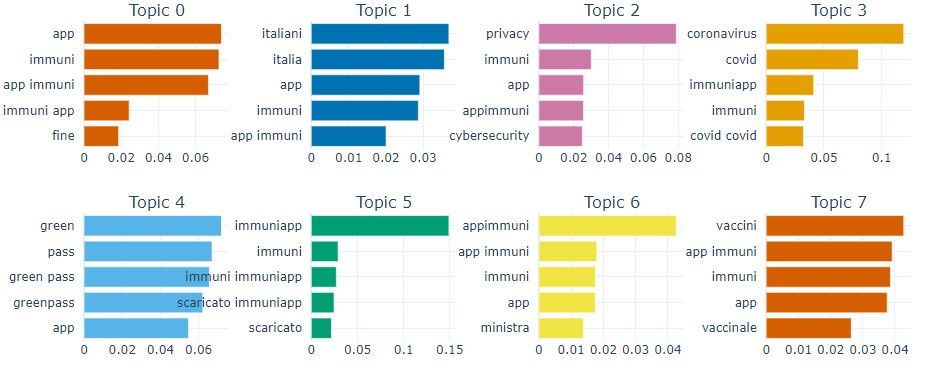
\includegraphics[width = 1\textwidth]{img/topics_tot.jpg}
    \caption{Argomenti più frequenti all'interno di tutti i tweet raccolti}
    \label{fig:topicMtot}
\end{figure}

Riguardo ai 10 temi estratti sul totale dei tweet (Figura \ref{fig:topicMtot}, è possibile notare come ci siano 3 diverse categorie di temi disposte secondo una gerarchia: quelli legati all'app in generale, quelli legati al green pass, alla privacy e alla sicurezza, tutti collegati al macro tema corrispondente al Topic 0 ossia il Coronavirus.

Analizzando invece i temi estratti dai tweet pubblicati nel 2020 e nel 2021 è possibile notare alcune differenze. 
\begin{figure}[H]
	\centering
	\subfloat[]
	{
		\label{topics_2020}
		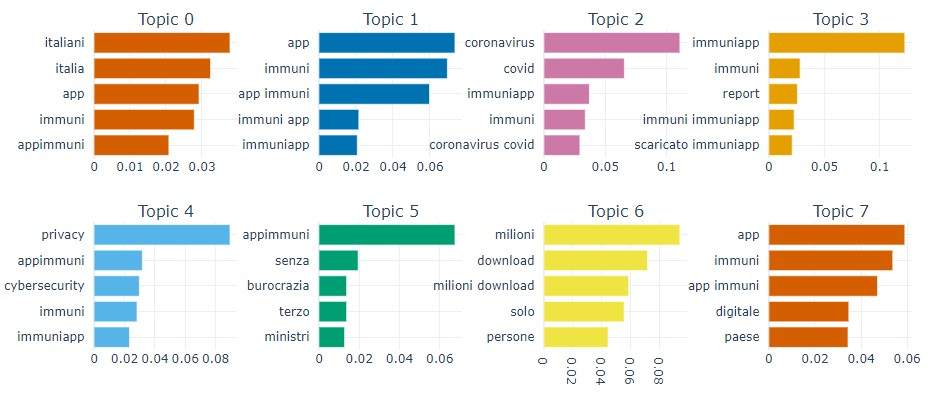
\includegraphics[width= 1\textwidth]{img/topics_2020.jpg}
	}
	\quad
	\subfloat[]
	{
		\label{topics_2021}
		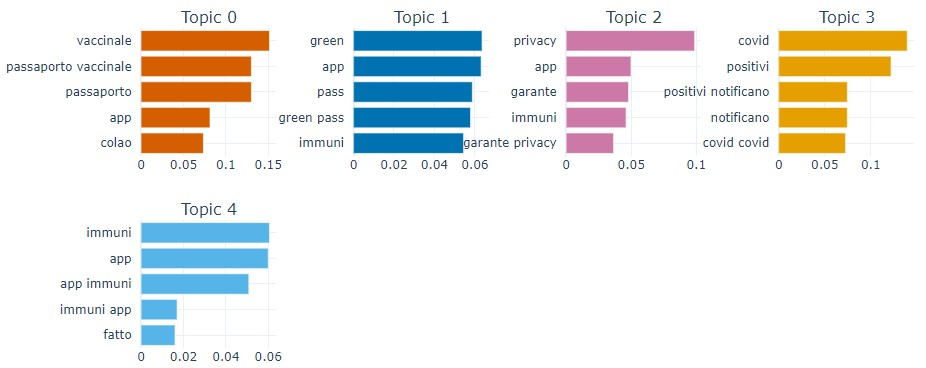
\includegraphics[width=1\textwidth]{img/topics_2021.jpg}
	}    
	\quad
	\setlength{\belowcaptionskip}{-10pt}
	\caption{Argomenti più ricorrenti nei tweet scritti nel 2020 (\ref{topics_2020}) e nel 2021 (\ref{topics_2021})}
	\label{fig: topicModels}
\end{figure}
La prima riguarda il numero di argomenti estratti, undici nel caso dei tweet scritti nel 2020 e sei nel caso di quelli scritti nel 2021, un aspetto che può essere giustificato dalle diverse dimensioni dei due insieme di dati (1107 tweet scritti nel 2020 e 473 nel 2021), mentre riguardo alla tipologia di temi individuati si nota come mentre nel 2020 (Figura \ref{topics_2020}) i temi più ricorrenti siano legati al Coronavirus e a Immuni, in cui emergono anche qui temi come la privacy, ma anche temi come i download e la burocrazia, nel 2021 (Figura \ref{topics_2021}), la discussione su Immuni è incentrata verso due temi molto influenti in quell'anno, ossia il Green Pass e la campagna vaccinale, rappresentati rispettivamente dal Topic 0 e Topic 1 in cui compaiono termini come appunto \textit{greenPass}, il quale viene indicato anche con il termine \textit{passaporto vaccinale}.

Da quest'ultima analisi emerge quindi nuovamente questa evoluzione dei temi trattati dagli utenti che dopo un iniziale interesse verso Immuni a causa dei forti contagi e della totale assenza di misure di prevenzione sufficientemente efficaci nel 2020, estendono nell'anno successivo la discussione sull'applicazione anche verso altri temi di tendenza come i vaccini e il Green Pass.
Tuttavia, il tema della privacy e della cessione dei dati continua ad essere un tema centrale in entrambi i periodi, sintomo che forse quello potrebbe essere uno dei problemi centrali che ha causato il graduale fallimento di Immuni.
